\chapter{Theoretical Background}
% \thispagestyle{fancy}
In this chapter, we provide a detailed description of the background of the degree project is presented along with related work. The background covers the autoencoder, which describes the fundamental behaviour of the later chosen network. Additionally, we present a general overview of Spiking Neural Network (\ac{SNN}) architectures and design choices.

\section{Related Work}
Spiking neural networks for control have found application in various contexts, including robotic movement, digit recognition\cite{lee_training_2016}, and object detection\cite{soures_deep_2019,zhou_deep_2020}.\\
In \cite{bouganis_training_2010}, spiking neurons are utilized to control target-reaching movements of a 4-DoF robotic arm using a plausible neuron model and learning rule. Their approach incorporates the DIRECT model from \cite{bullock_self-organizing_1993}, which learns the a priori unknown robot kinematics by randomly repeating movement commands and learning the resulting translation of the end effector.\\
Another approach for robotic arm control is presented in \cite{dewolf_spiking_2016}, utilizing the \ac{NEF}\cite{eliasmith_neural_2004}. Different regions of the brain are simulated to generate the trajectory and control signals. On the other hand, the authors of \cite{liu_spiking_2023} used \ac{RL} in combination with a \ac{SNN} and a variation of the \ac{STDP} rule to control the cart-pole problem.\\
The authors in \cite{bing_supervised_2019} summarized several approaches for robotic control of flying or driving robots and used layered spiking neurons with a local learning rule to train the network to reach the target while avoiding obstacles.\\
While each of these models incorporate some biological plausibility, they only take one or a few aspects into their model, be it the neuron model, the learning rule, encoding or network structure. Furthermore, these approaches are often targeted towards specific applications like robotic arms and may not address general control of dynamic systems.\\
Spiking neurons have also been explored for PID controllers. In \cite{lu_spiking_2011} it is demonstrated that a PID controller is possible using three neurons, each representing P,I and D, respectively. However, no example using the network is provided, and the learning process relies on individual parameter tuning for each neuron. Moreover, the robustness of 3 neurons is not biologically plausible.\\
In \cite{stagsted_towards_2020}, a PID controller is designed using spiking neurons on neuromorphic hardware in order to control a 1-DoF UAE.\\
However, details on how the network was trained on the neuromorphic hardware or how this approach can be scaled to larger systems remain unclear.\\
Additionally, due to the prevalent background noise found in the brain, we stride for a noise robust solution which is not given in any of the above mentioned approaches.\\
In addition to the individually crafted models by authors, various public libraries and frameworks have been developed in order to facilitate \ac{SNN} simulation. It is important to note that different libraries serve different purposes. While some to act as hybrids for \ac{SNN} with \ac{ML} goals (e.g. snnTorch\cite{eshraghian_training_2023}, nengo \cite{bekolay_nengo_2014}), others are geared for fast and accurate neurologic simulations (e.g. Brian\cite{stimberg_brian_2019}). Each framework implements a different feature set such as \ac{GPU} Support, Torch-like structure, convolution, learning rules, or support for neuromorphic hardware. For a summary, refer to  \cite{yamazaki_spiking_2022}.

\section{Autoencoder}
An autoencoder is a type of neural network designed to learn a representation of an input signal. It comprises an encoder and decoder function $z =f(x)$ \& $\hat{x} = g(z)$. The encoder function maps from the input space, for example $\mathbb{R}^n$, to an encoded space $\mathbb{Z}$. Subsequently, the decoder reconstructs the data from $\mathcal{Z}$ back to $\mathbb{R}^n$. The primary objective is to ensure that the decoded representation is as accurate as possible.\\
In the trivial case where $\mathcal{Z}$ is equal to or larger than the input space, each possible input can be encoded by its own value as
\begin{equation}
\begin{aligned}
 	z = f(x) &= x\\
 	\hat{x} = g(z) &= z = x
\end{aligned}
\end{equation}
and the autoencoder essentially memorizes each input. However, in most cases, $\mathcal{Z}$ is constrained, forcing the autoencoder to find the characteristic properties of the input. This is achieved by reducing the dimension of $\mathcal{Z}$ or through regularization. The regularization term, denoted as $C(z)$, is added to the Loss
\begin{equation}
	\tilde{L} = L(x,\hat{x}) + C(z)
\end{equation}
where L can be, for example, MSE. Regularization can enforce sparsity or other desired properties\cite{goodfellow_deep_2016}.\\
The functions $f$ and $g$ can be selected freely but play a crucial role in the performance. Frequently, they are combined in a neural network that is trained to adjust the network's parameters as well as function parameters. Additionally, the internal mechanism can also be freely chosen. Therefore, an autoencoder can also have a \ac{SNN} at its core, where $f$ and $g$ serving as the encoder and decoder of spikes, respectively.\\
This step is a pivotal aspect of the selected network architecture, essentially functioning as an autoencoder with spiking neurons. At each time step, a signal is encoded into a group of neurons, and the spiking dynamics are decoded to reconstruct the desired signal and each neuron projection different segments of the autoencoder's error.\\

\section{Neural Networks}
The topic of \acp{NN} is vast and has been extensively explored in numerous papers. In this section, we focus on design choices in neural networks and dedicated spiking models from the literature.\\
When designing a spiking neural network, various components must be selected to form the network. The following sections highlight the most crucial aspects and explain common choices. It is worth noting that \acp{SNN} are still under active research, many hybrids and combined methods exist, though they are not covered here.\\
\subsection{Spiking Neural Network Choices}

Copying nature to solve engineering problems is long-standing practise, and also extends to \acp{NN}. Numerous network architectures with varying levels of biological plausibility have been investigated and published, with little consent in design decisions. As a result different choices are made by different researches leading to various approaches that are similar yet different.\\
Biological realism can be incorporated at various points within the network, making it impractical to explicitly inspect each nuance. Apart from highly specific implementations illustrated in \cref{sec:spiking-neural-networks}, many \acp{SNN} can be categorized into different segments, showcasing certain designs found in the literature.\\
\subsubsection{Neuron model}
As outlined in more detail below, neuron models can vary in complexities and accuracy. By far, the most used model in the literature are \ac{LIF} and \ac{IF} models.\\

	\paragraph{Biological Neuron model}
	The first biologically accurate model of neuron spiking behaviour is the \ac{HH} model from 1952\cite{hodgkin_currents_1952}. Since then the \ac{HH} model has been extended in multiple ways to cover additional factors, such as different ion channels. The \ac{HH}-model considers the neuron with its ion channels. The membrane acts as a capacitance and the travelling ions in each ion channel contribute a current to the overall membrane potential. These ion gates are voltage-dependent and are defined positive in direction out of the cell.\\
	A particular ion channel for ion $X$ can be modelled as
	\begin{equation}
	I_X= g_X \cdot (V-V_X)
	\end{equation}
	These currents are summed for the different ion channels in question, most frequently for Sodium, Potassium and a leak current. In reality there is a plethora of different channels and channel properties\footnote{See  \url{channelpedia.epfl.ch} for an extensive list}. The $V_X$ are the equilibrium potentials for each of the channels and can be computed using the Nernst equation \cite{johnston_foundations_1995}.
	\begin{equation}
	C \frac{dV}{dt} = g_{Na} \cdot (V-V_{Na}) + g_K \cdot (V-V_K) + g_l \cdot (V-V_l)
	\end{equation}
	To model the voltage dependency of the ion channels, the conductances are described with gating variables, typically denoted as $n$, $m$ and $h$ for activation and inactivation of Sodium and Potassium channels. One gating variable is set between $[0,1]$ and models the permeability of a gate. Multiple gates are employed to match experimental data and model behaviour for each ion channel.\\
	Gates are modelled with order dynamics of the form
	\begin{equation}
	\frac{dn}{dt} = \alpha_n(1-n) - \beta_n n
	\end{equation}
	for the n gate. The other gates' dynamics are analogous. The functions $\alpha$ and $\beta$ are voltage but not time dependent. The discussion of initial values as well as functions for $\alpha_p,\ \beta_p\ \ p = (n,h,m)$ can be found in \cite{hodgkin_quantitative_1952} or \cite{johnston_foundations_1995}. The gates' conductance for each ion channel have been derived from natural approximations as follows:
	\begin{equation}
	\begin{aligned}
	g_{Na} &= \bar{g}_{Na} n^4\\
	g_{K} &= \bar{g}_{K} m^3h\\
	\end{aligned}
	\end{equation}
	and give form to the final model
	\begin{equation}\label{eq:HH}
	\begin{aligned}
	C\frac{dV}{dt} &= I(t) -\bar{g}_{Na} n^4(V-V_{Na}) - \bar{g}_{K} m^3h(V-V_{K}) -g_L(V-V_{L})\\
	\frac{dn}{dt} &= (1-n)\alpha_n(V) - \beta_n n (V)\\
	\frac{dm}{dt} &= (1-m)\alpha_m(V) - \beta_m m (V)\\
	\frac{dh}{dt} &= (1-h)\alpha_h(V) - \beta_h h (V).
	\end{aligned}
	\end{equation}
	We did not define a gate for the leak term as it is assumed constant.
	\paragraph{IF and LIF}
	In contrast to the \ac{HH} model in \cref{eq:HH}, the simplest models of neurons are the \ac{IF} and \ac{LIF} models.\\
	\subparagraph{IF Neurons}
	\ac{IF} Neurons, as the name implies, integrate the incoming current over time:
	\begin{equation}
	\frac{d V(t)}{d t} = \frac{1}{C}I(t)
	\end{equation}
	The membrane voltage is governed by the incoming current spikes of connected neurons and the membrane capacitance. The neuron potential does not change without a change of input current and thus presents itself as a perfect integrator of the input.\\
	\subparagraph{\ac{LIF} Neurons}
	In contrast, the \ac{LIF} neuron contains a leak term on the \ac{RHS}, bringing the voltage back to its resting potential over time. The model can be expressed as:
	\begin{equation}
	\tau\frac{dV(t)}{dt} = -(V(t)-E_r) + RI(t),
	\end{equation}
	where $\tau = RC$ is the time constant the composed of the membrane resistance $R$ and the membrane capacitance $C$. In the absence of input $I(t)$, the voltage settles on the membrane potential $E_r$.\\
	The input $I(t)$ encapsulates external inputs as well as a sum of Dirac functions indicating a firing neuron:
	\begin{equation}
	I(t) = \sum_k w_i\delta(t-t^k_i)
	\end{equation}
	Every received spike $k$ is multiplied by its respective synaptic strength from neuron $i$ and added to the input current. When the membrane voltage exceeds the threshold potential $\bar{V}$, a spike is sent out by the neuron and the voltage sets back to its reset voltage $V_{res}$.
	\paragraph{Izhikevich Neuron}
	While the above models deliver a useful and cheap model, they lack in accuracy. The Izhikevich model \cite{izhikevich_simple_2003} of the neuron aims to be a blend of efficiency and accuracy. It is comprised of 2D ODEs with the membrane potential $v$ defined as
	\begin{equation}
	\begin{aligned}
	\frac{d v}{dt} &= 0.04v^2 + 5v + 140 -u +I(t)\\
	\frac{d u}{dt} &= a(bv-u).
	\end{aligned}
	\end{equation}
	With the chosen factors, the neuron experiences a spike when $u\geq30 $mV, in which case the neuron resets to
	\begin{equation}
	\begin{aligned}
	u &\leftarrow u+d\\
	v&\leftarrow c.
	\end{aligned}
	\end{equation}
	The parameters describe $a$ as the scale of recovery, $b$ as sensitivity, $c$ as the reset potential of $v$, and $d$ as the reset of variable $u$. Depending on these parameters, one can achieve different behaviours of the neuron, such as regular spiking, fast spiking, and low threshold spiking to name a few.

\subsubsection{Encoding}
	The coding of information plays an important role in a \ac{SNN}. Since the network works with discrete spikes, a methodology needs to be implemented to convert e.g continuous values into spikes. To let the network be susceptible to the outer world, a subset of neurons of the network are exposed to these external inputs.
	\paragraph{\ac{TTFS}}
	In this coding scheme, the information of an input is solely encoded in the time between the external input and the time neurons fire a spike. A simple visualization could be by implementing such that the stronger the input, the sooner the input neuron spikes after the input onset.\\
	An extension of this idea is rank order coding, where the ordering of spikes encodes information\cite{thorpe_spike-based_2001}.\\
	\paragraph{Phase coding}
	Phase coding is a slight variation of the \ac{TTFS} code. Certain areas of the brain exhibit oscillations similar to a clock\cite{jacobs_critical_2013}. The premise of phase coding is that the oscillation of this clock can be used to convey information. Thus, a spike relative to the phase of a clock cycle entails information on the input signal.\\
	\paragraph{Rate coding}
	Rate coding transforms the intensity of a signal into a spiking pattern with a corresponding frequency. The intensity is often normalized to realistic spiking frequencies. Since the brain is noisy, the spike is not fired with the respective rate but rather with a Poisson process given a suitable rate $\lambda$.
	Using a Poisson point process comes with the drawback of comparatively high spiking rates to represent a value accurately due to noise\cite{deneve_efficient_2016}.
	\paragraph{Population coding}
	Population coding extends neuron encoding to multiple neurons. Instead of one neuron firing, a group of neurons is combined to encode information. This allows for redundancy and robustness. Inside this population, information can be embedded in different dynamics of this group. One way could be to consider the firing rate of the neurons as a group. Alternatively, pattern analysis can be performed to read out information in the distribution of spikes in the group.\\

\subsubsection{Connectivity/Topology}
	The structure of neural networks is mainly distinguished between hierarchical and recurrent topologies. In hierarchical topologies, there are segments of neurons that follow a (often unidirectional) structure. Feed-forward \acp{NN} are a simple example of this architecture.\\
	Recurrent networks allow for loops in the connectivity of neurons and therefore enable feedback and temporal patterns.\\
	There can be hybrid implementations where different groups of neurons are connected in sequence.\\
	Using \acp{RNN} offers a broader range of applications but has to deal with (as of this day) inferior or more complex learning paradigms.\\

\subsubsection{Plasticity}\label{sssec:plasticity}
	The choice of plasticity determines how the network adapts its parameters during learning. In the literature, mostly two different approaches are used. The dominant of these is the adjustment of synaptic weights, similar to \acp{ANN}. It is noteworthy that most learning algorithms are based on this approach.\\
	The alternative is to work on adjusting thresholds instead\cite{chen_adaptive_2022,amin_automated_2021}. One can adjust the frequency or likelihood of a neuron firing by lowering or increasing its threshold, making it harder or easier for a neuron to spike. Increasing the threshold after a spike was fired allows for the modelling of refractory periods seen in biological neurons.\\
	Threshold adaptation can also be in conjunction with weight adaption policy. In \cite{sun_synapse-threshold_2023}, adaptive synapses are trained alongside connection weights.\\
	Another form of plasticity concerns the retention of knowledge. In most \ac{ML} applications, the learning is solely a part of the deployment of a \ac{NN}. After the training period, the network parameters are fixed and further learning is frozen. This is in opposition to biological neural networks, where continuous learning is found not only due to the fact of neurons dying and getting replaced continuously but also due to the learning of new tasks.\\
	\acp{ANN} struggle with adjusting to new tasks while retaining the same performance for previous tasks. Since the learning of the new task is allowed to adjust every weight, it completely ignores relevant weights for the previous task.\\
	To combat this different ideas have been suggested. These include fixing parts of the weights, using Drop-Outs, or employing \ac{EWC}\cite{kirkpatrick_overcoming_2017}. In \ac{EWC}, crucial weights are retained by augmenting the cost function with a penalization term on the parameters deviation from the previous task. The proportional factors are computed using the Fisher information matrix after the learning of one task is completed and focus crucial neurons with higher proportional factors.\\
	A similar approach has been proposed with synaptic intelligence\cite{zenke_continual_2017}.
	Here, a similar penalty term is introduced that computes the neurons individual importance. The difference is that this importance can be computed online. Each synapse tracks a scalar value describing the relative importance of decreasing the loss. This value is the base for the importance calculation that again penalizes deviations of parameter weights from the previous values.\\
	However, as of now, this has only been implemented on \acp{ANN} with a Feed-forward architecture.

\subsubsection{Learning Algorithms}
	Key to giving any \ac{NN} the ability to solve a task is to learn/train the it. The adaptation of weights and biases is necessary to accomplish any functionality based on the underlying data\cite{zheng_introductory_2022}. There are a plethora of different learning techniques available; see \cite{abdolrasol_artificial_2021,sun_survey_2019} for a review. The most fundamental distinction can be made between supervised, unsupervised, and reinforcement learning rules. Another distinction can be made by the biologic plausibility of a given learning rule. For example, for \ac{ANN} the gradient based Backpropagation algorithm is biologically implausible in various ways, but most importantly in its non-locality, yet it has been immensely successful.\\
	In this context, a loss function $L$ is employed to calculate the derivative $\frac{\partial L}{\partial \theta_{ij}}$, determining the contribution of each neuron's parameters $\theta_{ij}$ to the error. Subsequently, these parameters are adjusted iteratively until a minimum is reached. The computation of gradients is done efficiently using the backpropagation algorithm (reverse accumulation from \ac{AD}), in which the gradients are propagated from the output backward towards the input by making use of the chain rule and the fact that the \ac{NN} has a layered structure. An in-depth explanation is given in, for example, \cite{goodfellow_deep_2016} or \cite{nielsen_neural_2015}.\\
	If the chosen network is recurrent, using \ac{BP} to find gradients is more complex. To remedy this, adaptations of the classic \ac{BP} algorithm have been proposed.\\
	For recurrent networks, often the \ac{BPTT} can be used. Its concept is based on using the conventional Backpropagation algorithm by "unrolling" the recurrent network into a feed-forward network in time. In addition to the original network inputs, additional inputs are designated in the feed-forward network that feed the internal network state to the next layer, representing the next time step.\\
	With this structure in place, the gradients can now be computed either by propagating the error backward or by forward propagation of the activity gradient. The former is commonly known as the normal \ac{BPTT} the latter is called \ac{RTRL}\cite{williams_gradient-based_1995}. While they allow the computation of the exact gradients, they can both suffer from issues like vanishing or exploding gradients \cite{pascanu_difficulty_2013,bengio_learning_1994} resulting in getting trapped in local minima easily or divergence. This is due to the unrolling in time, which causes the network to become deep quickly. For each step of the input sequence fed into the network, an extra layer in the unrolled network is added.\\
	Gradient-based methods require differentiability and therefore continuity, making them applicable only for \acp{ANN}. This means that they cannot be used for \acp{SNN} as spikes introduce discontinuities. Since spikes are discrete events the derivative is zero during no-spike periods and undefined during a spike.\\
	While methods have been proposed to adapt backpropagation to spiking networks\cite{lee_training_2016}, they still lack a biologically plausible way to learn. The problem is that in biology, neurons do not have access to the global error from the loss function but only receive information from pre-synaptic neurons.\\
	For spiking and recurrent networks, the \ac{BPTT} algorithm can be combined with spiking networks, leading to the SpikeProp\cite{bohte_spikeprop_2000} algorithm. In SpikeProp, the optimization is performed on the firing times, and the discontinuity is replaced by a linear function. Several variations have emerged with improved convergence\cite{mckennoch_fast_2006}, e.g by using different replacement functions \cite{thiruvarudchelvan_analysis_2013,neftci_surrogate_2019} or adaptive learning weights \cite{shrestha_adaptive_2015}.
	Alternatively, instead of optimizing the firing times and replacing the discontinuity in spike trains, SuperSpike\cite{zenke_superspike_2018} replaces the discontinuities in the membrane potential with an approximate continuous function.\\
\paragraph{(Anti-) Hebbian Learning and STDP}
Tending towards more biologically plausible methods, \ac{STDP} is the most prominent method.\\
The Hebbian learning rule is one of the oldest learning principles for spiking networks with large experimental evidence in biology (see for example \cite{feldman_spike-timing_2012} for a summary). Its core idea can be encapsulated in the famous mnemonic "Neurons that fire together, wire together." Essentially, if the postsynaptic neuron repeatedly fires shortly after the presynaptic neuron, their connection strength is increased. Oppositely, if the postsynaptic neuron fires before the presynaptic, their connection strength is decreased.\\
This behaviour of potentiation and depression is illustrated in \cref{fig:stdp} and build the bases for the \ac{STDP} rule. It operates by increasing the synaptic weight of a synaptic connection when a presynaptic spike is followed by a postsynaptic spike, conversely, reducing the weight if the spikes occur independently, i.e. the postsynaptic neuron firing first. The longer the delay between firing activation, the smaller the increase.\\
Since then a plethora of variations have been proposed and demonstrated successfully\cite{vigneron_critical_2020,tavanaei_bp-stdp_2019,yamazaki_spiking_2022}.
\begin{figure}
	\centering
	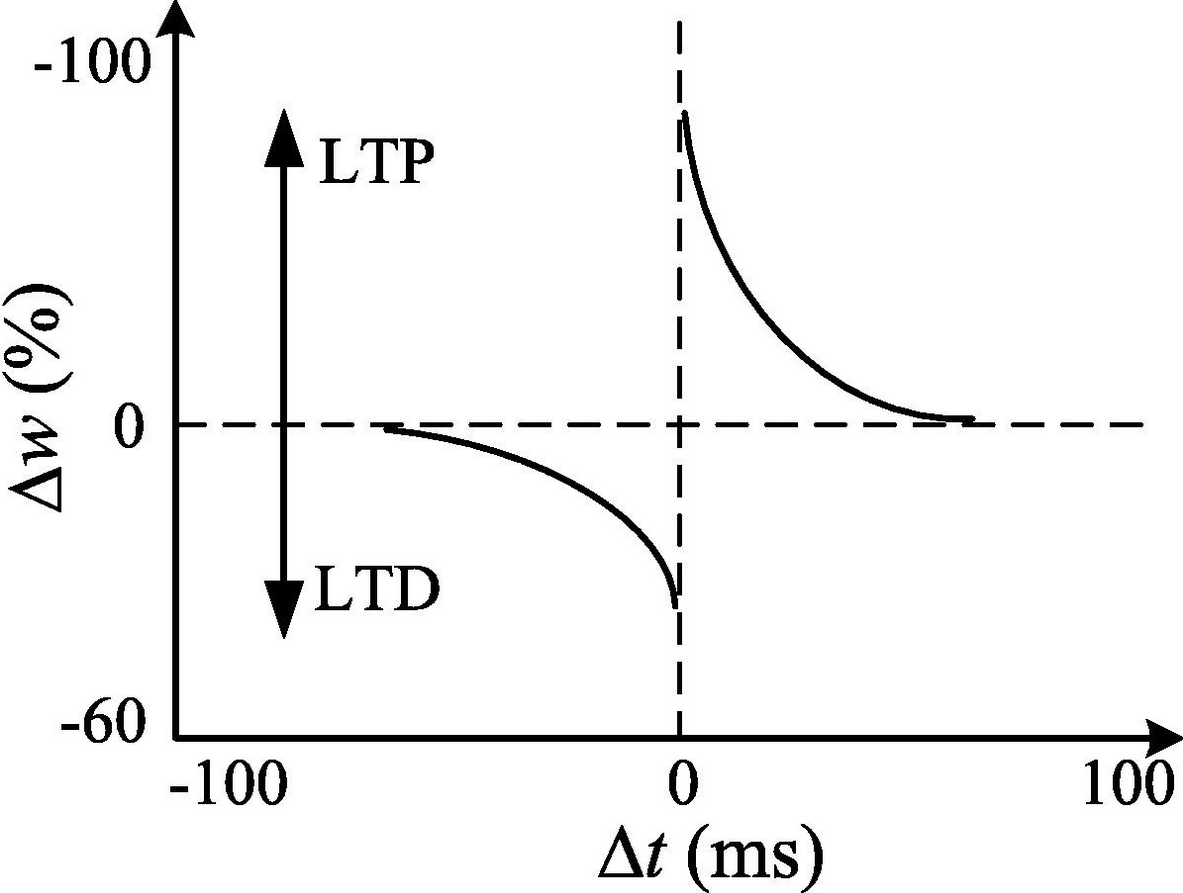
\includegraphics[scale = 0.15]{stdp}
	\caption{Graphical representation of STDP learning rule. Weight change depending on the time between pre- and postsynaptic activation. Negative time is the time between the postsynaptic neuron firing before the presynaptic. Graphic taken from \cite{yi_learning_2023}.}
	\label{fig:stdp}
\end{figure}
In addition to the Hebbian rule, there is also the anti-Hebbian rule, which reverses the aforementioned behaviour. This implies that regular firing of pre- and postsynaptic neurons is discouraged and more irregular and distributed spiking is favoured. This can be understood as mirroring \cref{fig:stdp} along the x-axis.\\
Several variations and extensions to \ac{STDP} have been proposed, e.g. \ac{SRDP}\cite{kempter_hebbian_1999} or reward modulated \ac{STDP}\cite{legenstein_learning_2008}.

These rules are rooted in biology and adhere to the constraints observed in nature. Many learning rules adapted from \acp{ANN} lack these properties e.g. locality.\\
Locality dictates that the basis of learning is restricted to having only the information of the direct pre- and postsynaptic neurons available. This already rules out most backpropagation algorithms, as they derive the derivative with respect to a global cost function.


\subsection{Spiking Neural Networks}\label{sec:spiking-neural-networks}
Apart from the aforementioned segments of \acp{SNN}, various \ac{SNN} archetypes have been studied in the literature. In the following sections, rate networks and \acp{LSM} will be presented. Note that the following sections do not represent a comprehensive review but rather a selective overview options. In addition to the \ac{SNN} types mentioned below, other approaches exist, such as the \ac{NEF}\cite{eliasmith_neural_2004}, SORN\cite{lazar_sorn_2009}, or FORCE \cite{nicola_supervised_2017}.
\subsubsection{Rate Networks}
Poisson or Rate networks are built around the idea that information is encoded in the firing rate of a neuron. The precise timing of a spike is essentially meaningless\cite{brette_philosophy_2015}. This contrasts with the approach chosen in this project. While states are also decoded using neuron firing rates, each fired spike is times exactly in order to minimize a cost function.\\
The encoding of a value in rate networks, e.g. four, is set by endowing the input neurons with a Poisson point process with a suitable encoding rate $r_i$\cite{deneve_efficient_2016}.\\
One typically uses probabilistic stimuli because observations in the spiking of the human brain do are different in a trial-by-trial basis.\\
Input spikes traverse the recurrent network with weighted connections. The decoding is done by counting the spikes of output neurons over a certain time window. The time window plays a crucial role in the decoding. If it is set smaller, spatio temporal patterns can be captured which can convey information about the input. Equally the sensitivity to noise becomes higher. If the time window is set too large, the firing patterns are lost due to exceedingly large averaging, although the impact of random spikes is reduced.\\
Using this method is a comparatively simple way of encoding, as firing rates are used in favour of the individual spikes, which are modelled by random processes. Additionally, this approach is biologically not completely unsound. In nature, it has been shown that the firing rate does convey information about the stimuli's magnitude. \cite{adrian_impulses_1926}.\\
The connection weights are subject to change over the learning/training period\cite{almomani_comparative_2019} and can be trained with different training algorithms, e.g. (anti-)Hebbian, \ac{STDP}, gradient based or more involved training methods\cite{demin_recurrent_2018}. See \cite{yi_learning_2023} for an overview.\\


The challenge with a Poisson process generating spikes for its respective rate is that this process requires many spikes to accurately transmit a signal. For N neurons representing a given value, the error or variance scales with $\frac{1}{\sqrt{N}}$\cite{boerlin_predictive_2013}. In other words, to achieve accurate results, a substantial number of spikes must be fired. If the time between spikes follows an exponentially distributed pattern, and having a greater number of samples enhances the accuracy of estimating the rate parameter.\\
Theoretically, using a large number of spikes is unproblematic. Even with large spike counts, neuromorphic hardware is still highly energy efficient compared to deep neural networks when deployed\cite{indiveri_importance_2019}.\\


However, there are more issues to this method. This approach has the limitation that responses are confined by the time window in which spikes are counted\cite{andrew_spiking_2003}. This implies that the rate decoding may be insufficiently swift to capture rapidly propagating information\cite{guo_neural_2021}, necessitating the exploration of faster means to transmit information.\\
Despite the aforementioned challenges, rate-encoded \acp{SNN} have garnered interest in research. A significant hurdle in deploying \acp{SNN} is the lack of performant learning algorithms. Efforts have been made to train recurrent or convolutional \acp{ANN} using backpropagation and then convert the trained network afterwards to a \ac{SNN}\cite{pfeiffer_deep_2018} using rate encoding\cite{diehl_conversion_2016}\cite{diehl_fast-classifying_2015}.
&&
\subsubsection{Liquid state machines}
One alternative method that has been proposed is the use of \ac{LSM} or more general Reservoir computing.\\
The term Reservoir computing was introduced by Benjamin Schrauwen and describes a general group of recurrent network approaches\cite{verstraeten_experimental_2007}.\\
The "reservoir" is a non-linear map from input to outputs that combines the input in various, even random ways. These contain but are not limited to sums, differences, multiplications, division and exponentiation. In general the output $\bmu{x}(t)$ is higher dimensional that the input $\bmu{v}(t)$, in order to allow for sufficient variety in the mapping. The output of the reservoir, which is usually treated as a black box, is fed in a linear decoder in order to retrieve the desired output signal.\\
\begin{figure}
	\centering
	\includesvg[scale= 0.15]{reservoir_computing}
	\caption{Abstract idea of Reservoir Computing. Adapted from \cite{cooper_liquid_2011}}
	\label{fig:reservoir_computing}
\end{figure}
The liquid can be made of any system that fulfils two properties.\\
\begin{itemize}
	\item Non-linear nodes of computation
	\item Fading memory
\end{itemize}
To these points it is usually set for the system to be time invariant\cite{cooper_liquid_2011}.
A reservoir can be a mathematical abstract formulation or physical object, e.g. a literal bucket of water \cite{tanaka_recent_2019}.\\
After the choice of "liquid" in the reservoir is fixed, its dynamics are not altered. Only the linear decoder is trained to return the desired decoded output\cite{jaeger_echo_2010}. This is a considerable time saving since the training of recurrent networks is expensive. On the contrary the linear decoder can be learned relatively cheaply.\\
A reservoir computer is called a \ac{LSM} if one chooses a spiking neural network as the reservoir. The requirements mentioned above are fulfilled by the recurrent structure to retain information of the neurons and its non-linear spiking behaviour.\\
\acp{LSM} are capable of computing any dynamical system of any order of the form of
\begin{equation}
	z^{(n)} = G(z,z^{(1)},z^{(2)},\dots,z^{(n-1)}) + u
\end{equation}
given a sufficiently large liquid and a suitable feedback and decoder\cite{maass_computational_2004} and have been used for speech recognition\cite{jin_performance_2017}\cite{zhang_digital_2015} or object detection\cite{soures_deep_2019}. The systematic structure can be in seen in \cref{fig:LSM_feedback}. The feedback $K(x,u)$ is a function of the dynamical system input $u(t)$ and the output $x(t)$. The result of $K(x,u)$ is fed back replaces the previous input $v(t)$ into the Liquid. The decoder $h(x)$ is not linear but can be simplified to be in a cost-performance trade-off when using a sufficiently large Liquid.\\
\begin{figure}[htbp]
	\centering
	\includesvg[scale= 0.15]{LSM_feedback2}
	\caption{Adding suitable feedback allows \acp{LSM} to be universal approximator. Adapted from \cite{maass_computational_2007}}
	\label{fig:LSM_feedback}
\end{figure}

\subsubsection{Balanced Efficient Coding Networks}
The idea of tightly balanced spiking networks was first proposed by Boerlin et al.\cite{boerlin_predictive_2013}. It uses predictive coding in combination with spikes to simulate arbitrary linear or non-linear systems\cite{alemi_learning_2017}.
The technical derivation will be described in \cref{ssec:balanced_network_sim}. The approach defines a cost function measuring the networks' accuracy in addition with regularization terms that moderates the spiking behaviour. Using a greedy optimization algorithm this cost function determines the voltage threshold and therefore the neurons' spiking behaviour.\\
For each neuron voltage can be understood as a projection of the global system error to a local error. One neuron is only tracking the system error under this projection. When the error under this projection reaches a threshold, a spike is fired.\\
The firing of a neuron resets its voltage as well as correcting the system to reset the perceived projected error.\\

Balanced networks differ from the previous rate encoding in that excitation and inhibition is closely tracked. In rate encoded networks both inhibitory and excitatory spikes are received by a single neuron. An change of the variable is then governed by which type dominates. Here a rate coding is used, however in the matter of control, a combination with instantaneous decoding is \cite{johnson_minimum-error_2016} utilized. The difference to typical rate networks is given by the fact that each spike distinct information.\\
Each neuron's projects some information about the state and the network. By projecting the system error in different directions, we assign each neuron to track one projection error, identified with a neurons voltage. If a neurons voltage reaches the threshold, the projected error exceeds the threshold, a spike is fired and counteracting the projected error.\\
The projection of the system error therefore has immense influence on an individual neuron's spiking behaviour but also the whole network.\\
On the other hand in rate networks, a population of neurons is given a value to represent and the population spiking rate encodes this value. An individual spike in this population does not have a direct relevance to the system and a discrete impact on its behaviour.\\
